\section{Data transformation and data discretization}

\begin{frame}{Data Transformations}
	\begin{itemize}
		\item Functions applied to a finite set of samples.
		\item \textbf{Methods:}
		      \begin{itemize}
			      \item Smoothing: Remove noise from data.
			      \item Attribute/feature construction: New attributes constructed
			            from the given ones.
			      \item Aggregation: Summarization, data-cube construction.
			      \item Normalization: Scaled to fall within a smaller, specified
			            range.
			            \begin{itemize}
				            \item Min-max normalization
				            \item Z-score normalization.
				            \item Normalization by decimal scaling.
			            \end{itemize}
			      \item Discretization: concept-hierarchy climbing.
		      \end{itemize}
	\end{itemize}
\end{frame}

\begin{frame}{Normalization}
	\begin{itemize}
		\item \textbf{Min-max normalization (to some interval
			      $[\text{min},\text{max}]$):}
		      \begin{align*}
			      a_{\text{new}} = \frac{a - \text{min}_A}{\text{max}_A-\min_{A}}
			      (\max - \min) + \min.
		      \end{align*}
		      Example: let income range from $\$12,000$ to $\$98,000$ normalized to
		      $[0,1]$.\\
		      Then $\$73,600$ is mapped to $\frac{73,600-12,000}{98,000-12,000} (1-0)
			      + 0 = 0.716$.
		\item \textbf{Z-score normalization:}
		      \begin{align*}
			      a_{\text{new}} := z(a) = \frac{a-\mu_{A}}{\sigma_A}, \; \text{with
				      $\mu$ being the mean and $\sigma$ the standard deviation.}
		      \end{align*}
		      Example: let $\mu = 54,000$ and $\sigma = 16,000$. Then
		      $\frac{73,000-54,000}{16,000} = 1.188$.
		\item \textbf{Normalization by decimal scaling:}
		      \begin{align*}
			      a_{\text{new}} = \frac{a}{10^k}, \; \text{where $k$ is the smallest
				      integer such that} \; \max(\vert a_{\text{new}} \vert) < 1.
		      \end{align*}
	\end{itemize}
\end{frame}

\begin{frame}{Discretization}
	\begin{itemize}
		\item \textbf{Three types of attributes:}
		      \begin{itemize}
			      \item Nominal -- values from an unordered set, e.g. color,
			            profession.
			      \item Ordinal -- values from an ordered set, e.g. military or
			            academic rank.
			      \item Numerical -- numbers, e.g. integer or real numbers.
		      \end{itemize}
		\item \textbf{Divide the value range of a continuous attribute into
			      intervals:}
		      \begin{itemize}
			      \item \textbf{Interval labels} can then be used to replace actual
			            data values.
			      \item Reduce data size by discretization.
			      \item Supervised vs. unsupervised.
			      \item Split (top-down) vs. merge (bottom-up).
			      \item Discretization can be performed recursively on an attribute.
			      \item Prepare for further analysis, e.g. classification.
		      \end{itemize}
	\end{itemize}
\end{frame}

\begin{frame}{Data-discretization Methods}
	\begin{itemize}
		\item \textbf{Typical methods:}
		      \begin{itemize}
			      \item All the methods can be applied recursively.
			      \item \textbf{Binning:}
			            \begin{itemize}
				            \item Unsupervised, top-down split.
			            \end{itemize}
			      \item \textbf{Histogram analysis:}
			            \begin{itemize}
				            \item Unsupervised, top-down split.
			            \end{itemize}
			      \item \textbf{Clustering analysis:}
			            \begin{itemize}
				            \item Unsupervised, top-down split or bottom-up merge.
			            \end{itemize}
			      \item \textbf{Decision-tree analysis:}
			            \begin{itemize}
				            \item Supervised, top-down split.
			            \end{itemize}
			      \item \textbf{Correlation (e.g. $\chi^2$) analysis:}
			            \begin{itemize}
				            \item Unsupervised, bottom-up merge.
			            \end{itemize}
		      \end{itemize}
	\end{itemize}
\end{frame}

\begin{frame}{Simple Discretization: Binning}
	\begin{itemize}
		\item \textbf{Equal-width (distance) partitioning:}
		      \begin{itemize}
			      \item Divides the range into $N$ intervals of equal size: uniform
			            grid.
			      \item If $A$ and $B$ are the lowest and highest values of the
			            attribute, the width of intervals will be: $W = \frac{(B - A)}{N}$.
			      \item The most straightforward, but outliers may dominate
			            presentation.
			      \item Skewed data is not handled well.
		      \end{itemize}
		\item \textbf{Equal-depth (frequency) partitioning:}
		      \begin{itemize}
			      \item Divides the range into $N$ intervals, each containing
			            approximately the same number of samples.
			      \item Good data scaling.
			      \item Managing categorical attributes can be tricky.
		      \end{itemize}
	\end{itemize}
\end{frame}

\begin{frame}{Binning Methods for Data Smoothing}
	\begin{itemize}
		\item \textbf{Sorted data for price (in dollars):} \\
		      $4, 8, 9, 15, 21, 21, 24, 25, 26, 28, 29, 34$.
		\item \textbf{Partition into equal-frequency (equal-depth) bins:}\\
		      Bin $1$: $4, 8, 9, 15$,\\
		      Bin $2$: $21, 21, 24, 25$,\\
		      Bin $3$: $26, 28, 29, 34$.
		\item \textbf{Smoothing by bin means:}\\
		      Bin $1$: $9, 9, 9, 9$,\\
		      Bin $2$: $23, 23, 23, 23$,\\
		      Bin $3$: $29, 29, 29, 29$.\\
		\item \textbf{Smoothing by bin boundaries:}\\
		      Bin $1$: $4, 4, 4, 15$,\\
		      Bin $2$: $21, 21, 25, 25$,\\
		      Bin $3$: $26, 26, 26, 34$.\\
	\end{itemize}
\end{frame}

\begin{frame}{Discretization without using Class Labels (Binning vs.
		Clustering)}
	\begin{figure}[H]
		\centering
		\begin{minipage}{0.32\textwidth}
			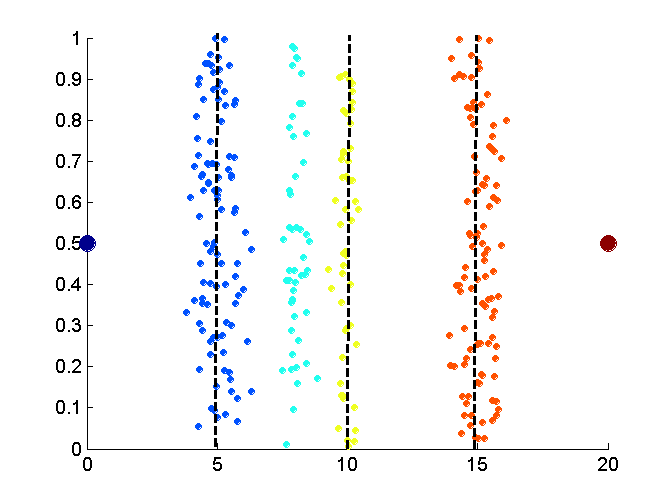
\includegraphics[width=5cm]{img/binningvsclustering2.png}
			\caption{a) Equal interval width (binning).}
		\end{minipage}
		\begin{minipage}{0.32\textwidth}
			\centering
			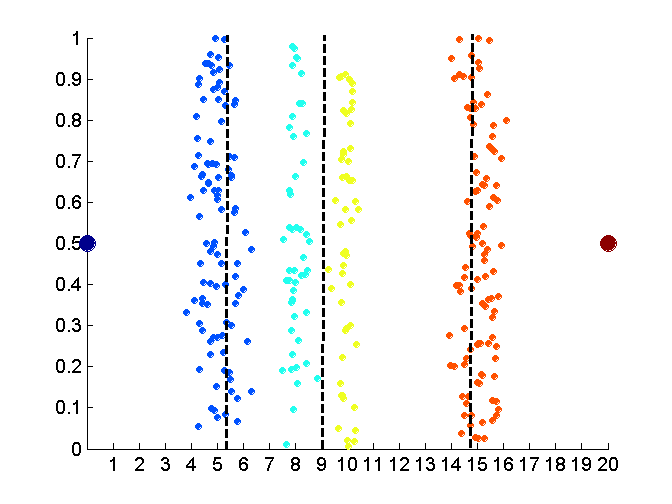
\includegraphics[width=5cm]{img/binningvsclustering3.png}
			\caption{b) Equal frequency (binning).}
		\end{minipage}
		\begin{minipage}{0.32\textwidth}
			\centering
			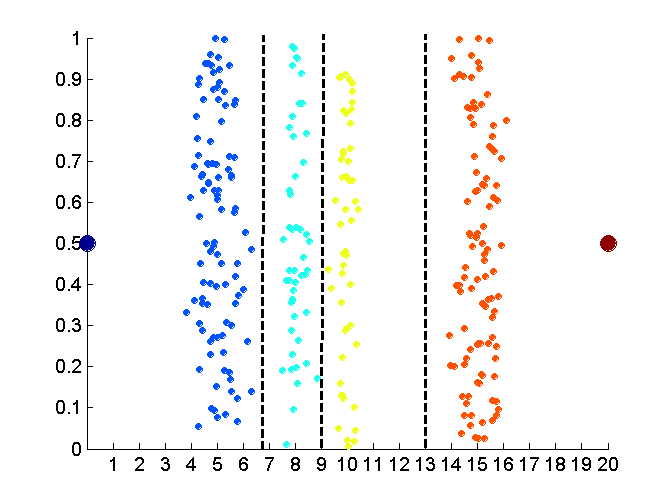
\includegraphics[width=5cm]{img/binningvsclustering4.png}
			\caption{c) K-means clustering.}
		\end{minipage}\hfill
	\end{figure}
\end{frame}

\begin{frame}{Discretization by Classification \& Correlation Analysis}
	\begin{itemize}
		\item \textbf{Classification:}
		      \begin{itemize}
			      \item E.g. decision-tree analysis.
			      \item Supervised: Class labels given for training set e.g.
			            cancerous vs. benign.
			      \item Using \textbf{entropy} to determine split point
			            (discretization point).
			      \item Top-down, recursive split.
			      \item Details will be covered in Chapter 6.
		      \end{itemize}
		\item \textbf{Correlation analysis:}
		      \begin{itemize}
			      \item E.g. $\chi^2$-merge: $\chi^2$-based discretization.
			      \item Supervised: use class information.
			      \item Bottom-up merge: find the best neighboring intervals (those
			            having similar distributions of classes, i.e., low $\chi^2$ values)
			            to merge.
			      \item Merge performed recursively, until a predefined stopping
			            condition.
		      \end{itemize}
	\end{itemize}
\end{frame}

\begin{frame}{Concept-hierarchy Generation}
	\begin{itemize}
		\item \textbf{Concept hierarchy:}
		      \begin{itemize}
			      \item Organizes concepts (i.e. attribute values) hierarchically.
			      \item Usually associated with each dimension in a data warehouse.
			      \item Facilitates \textbf{drilling and rolling} in data warehouses
			            to view data at multiple granularity.
		      \end{itemize}
		\item \textbf{Concept-hierarchy formation:}
		      \begin{itemize}
			      \item Recursively reduce the data by collecting and replacing
			            \textbf{low-level concepts} (such as numerical values for age) by
			            \textbf{higher-level concepts} (such as youth, adult, or senior).
			      \item Can be explicitly specified by domain experts and/or
			            data-warehouse designers.
			      \item Can be automatically formed for both numerical and nominal
			            data.
			      \item For numerical data, use discretization methods shown.
		      \end{itemize}
	\end{itemize}
\end{frame}

\begin{frame}{Concept-hierarchy Generation for Nominal Data}
	\begin{itemize}
		\item \textbf{Specification of a partial/total ordering of attributes
			      explicitly at the schema level by users or experts.}
		      \begin{itemize}
			      \item $\#(\text{streets}) \prec \#(\text{city}) \prec
				            \#(\text{state}) \prec \#(\text{country})$.
		      \end{itemize}
		\item \textbf{Specification of a hierarchy for a set of values by
			      explicit data grouping.}
		      \begin{itemize}
			      \item $\#(\{"Urbana", "Champaign", "Chicago"\}) \prec
				            \#(\text{Illinois})$.
		      \end{itemize}
		\item \textbf{Specification of only a partial set of attributes.}
		      \begin{itemize}
			      \item Only $\#(\text{street}) \prec \#(\text{city})$, not others.
		      \end{itemize}
		\item \textbf{Automatic generation of hierarchies (or attribute levels)
			      by the analysis of the number of distinct values.}
		      \begin{itemize}
			      \item E.g. for a set of attributes: $\{\text{street}, \text{city},
				            \text{state}, \text{country}\}$.
			      \item See on the next slides.
		      \end{itemize}
	\end{itemize}
\end{frame}

\begin{frame}{Automatic Concept-hierarchy Generation}
	\begin{itemize}
		\item \textbf{Some hierarchies can be automatically generated based on
			      the analysis of the number of distinct values per attribute.}
		      \begin{itemize}
			      \item The attribute with the most distinct values is placed at the
			            lowest level of the hierarchy.
			      \item Exceptions, e.g. weekday, month, quarter, year.
		      \end{itemize}
		\item Example:
		      \begin{align*}
			      \#(\text{streets})           & = 674.339 > \#(\text{city}) =
			      3567,                                                         \\
			      \#(\text{city})              & =  3567 > \#(\text{province or
			      state}) =  356,                                               \\
			      \#(\text{province or state}) & =  356 > \#(\text{country}) =
			      15.
		      \end{align*}
	\end{itemize}
\end{frame}
